% Schema del modello definito in 03_training.py, versione a 4 teste, disegnato
% nello stile della Figura 1 di "Attention Is All You Need" (di cui questo e'
% in pratica la meta' destra, il decoder, ridotta all'osso).
%
% Compilare con:
%     pdflatex 03_out_architecture.tex
%     tectonic 03_out_architecture.tex
%
% Per riusarlo dentro un altro documento: copiare le \definecolor, la lista di
% stili e il blocco tikzpicture, lasciando perdere il resto del preambolo.

\documentclass[tikz,border=8pt]{standalone}

\usepackage[T1]{fontenc}
\usepackage{lmodern}
\usetikzlibrary{positioning,fit,calc,arrows.meta,backgrounds}

% i colori pastello della figura originale
\definecolor{cEmb}{RGB}{248,214,216}
\definecolor{cAtt}{RGB}{252,224,187}
\definecolor{cFF}{RGB}{200,225,245}
\definecolor{cLin}{RGB}{216,214,238}
\definecolor{cSM}{RGB}{205,235,205}
\definecolor{cBlk}{RGB}{240,240,240}

\begin{document}
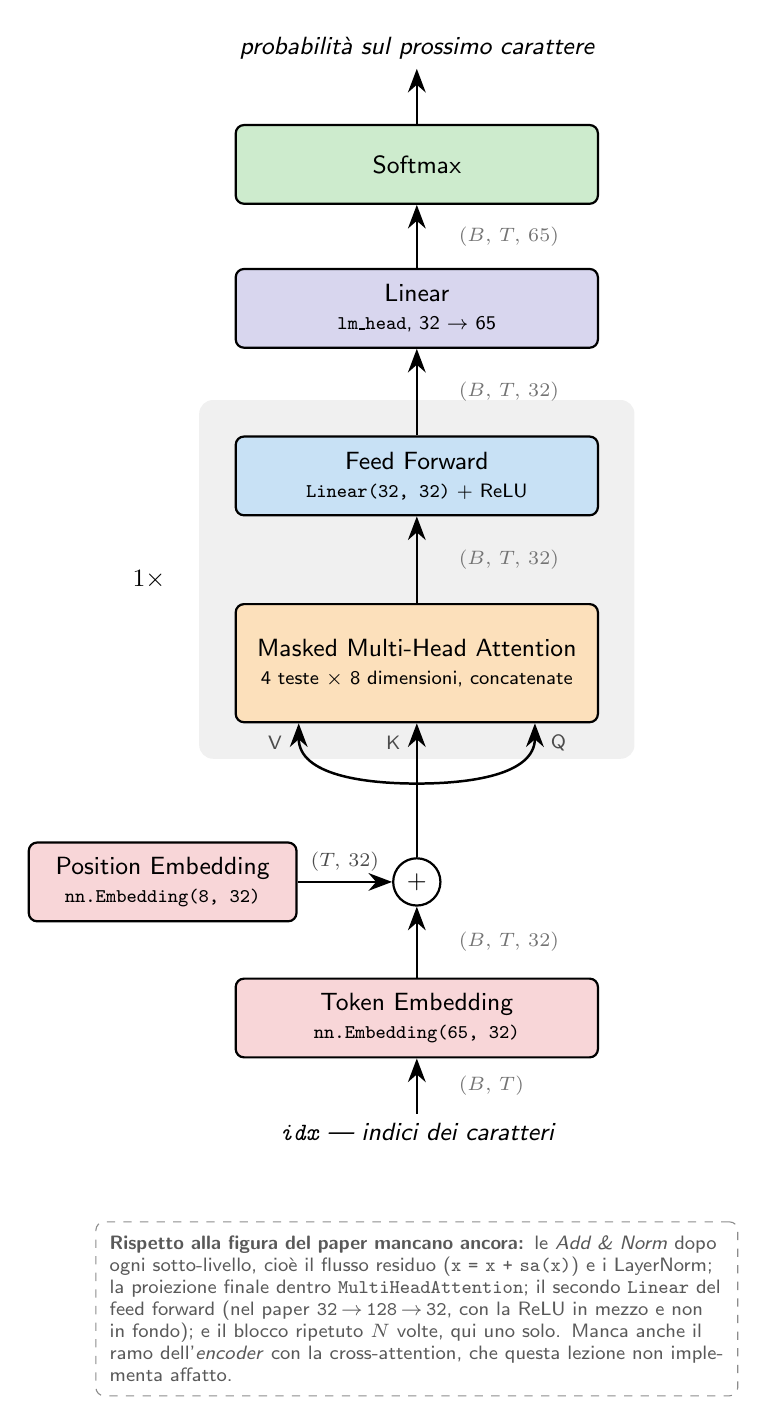
\begin{tikzpicture}[
  font=\sffamily\small,
  box/.style   = {draw, thick, rounded corners=3pt, align=center,
                  minimum width=46mm, minimum height=10mm, inner sep=3pt},
  io/.style    = {align=center, font=\sffamily\small\itshape},
  flow/.style  = {-{Stealth[length=3mm]}, line width=0.9pt},
  shp/.style   = {font=\sffamily\scriptsize, text=black!55,
                  anchor=west, xshift=4mm},
  qkv/.style   = {font=\sffamily\scriptsize, text=black!70},
  note/.style  = {draw=black!45, dashed, rounded corners=3pt, align=left,
                  font=\sffamily\scriptsize, text=black!65, inner sep=5pt}
]

% ---------------------------------------------------------------- il flusso --
\node[io]                                   (inp) {\texttt{idx} \textemdash{} indici dei caratteri};
\node[box, fill=cEmb, above=7mm of inp]     (tok) {Token Embedding\\[-1pt]{\scriptsize\texttt{nn.Embedding(65, 32)}}};
\node[draw, thick, circle, minimum size=6mm,
      inner sep=0pt, above=9mm of tok]      (add) {$+$};
\node[box, fill=cEmb, left=12mm of add,
      minimum width=34mm]                   (pos) {Position Embedding\\[-1pt]{\scriptsize\texttt{nn.Embedding(8, 32)}}};
\node[box, fill=cAtt, above=17mm of add,
      minimum height=15mm]                  (mha) {Masked Multi-Head Attention\\[-1pt]{\scriptsize 4 teste $\times$ 8 dimensioni, concatenate}};
\node[box, fill=cFF, above=11mm of mha]     (ff)  {Feed Forward\\[-1pt]{\scriptsize\texttt{Linear(32, 32)} + ReLU}};
\node[box, fill=cLin, above=11mm of ff]     (lm)  {Linear\\[-1pt]{\scriptsize\texttt{lm\_head}, 32 $\rightarrow$ 65}};
\node[box, fill=cSM, above=8mm of lm]       (sm)  {Softmax};
\node[io, above=7mm of sm]                  (outp) {probabilit\`a sul prossimo carattere};

% ------------------------------------------------------------------- archi --
\draw[flow] (inp) -- (tok) node[shp, midway] {$(B,\,T)$};
\draw[flow] (tok) -- (add) node[shp, midway] {$(B,\,T,\,32)$};
\draw[flow] (pos) -- (add) node[qkv, midway, above] {$(T,\,32)$};

% dal residuo alle tre proiezioni: ogni testa ricava K, Q, V dallo stesso x
\coordinate (split) at ($(add.north)!0.55!(mha.south)$);
\draw[line width=0.9pt] (add) -- (split);
\draw[flow] (split) to[out=180, in=-90] ([xshift=-15mm]mha.south);
\draw[flow] (split) --                  ([xshift=0mm]mha.south);
\draw[flow] (split) to[out=0,   in=-90] ([xshift=15mm]mha.south);
\node[qkv] at ([xshift=-18mm, yshift=-2.5mm]mha.south) {V};
\node[qkv] at ([xshift=-3mm,  yshift=-2.5mm]mha.south) {K};
\node[qkv] at ([xshift=18mm,  yshift=-2.5mm]mha.south) {Q};

\draw[flow] (mha) -- (ff) node[shp, midway] {$(B,\,T,\,32)$};
\draw[flow] (ff)  -- (lm) node[shp, midway] {$(B,\,T,\,32)$};
\draw[flow] (lm)  -- (sm) node[shp, midway] {$(B,\,T,\,65)$};
\draw[flow] (sm)  -- (outp);

% -------------------------------------------------- il "blocco", ripetuto 1x --
\begin{scope}[on background layer]
  \node[fill=cBlk, rounded corners=5pt, fit=(mha)(ff), inner sep=4.5mm] (blk) {};
\end{scope}
\node[font=\sffamily\small, left=3mm of blk] {$1\times$};

% -------------------------------------------------------------- cosa manca --
\node[note, below=9mm of inp, text width=78mm] (nota) {%
  \textbf{Rispetto alla figura del paper mancano ancora:} le \emph{Add \& Norm}
  dopo ogni sotto-livello, cio\`e il flusso residuo (\texttt{x = x + sa(x)})
  e i LayerNorm; la proiezione finale dentro \texttt{MultiHeadAttention};
  il secondo \texttt{Linear} del feed forward (nel paper
  \texttt{32\,$\to$\,128\,$\to$\,32}, con la ReLU in mezzo e non in fondo);
  e il blocco ripetuto $N$ volte, qui uno solo.
  Manca anche il ramo dell'\emph{encoder} con la cross-attention, che questa
  lezione non implementa affatto.};

\end{tikzpicture}
\end{document}
